\documentclass[journal,10pt,twocolumn]{article}
\usepackage{graphicx}
\usepackage[margin=0.5in]{geometry}
\usepackage{amsmath}
\usepackage{kvmap}
\usepackage{float}
\usepackage{lmodern}
\renewcommand*\familydefault{\sfdefault}
\usepackage{watermark}
\usepackage{karnaugh-map}
\usepackage{lipsum}
\usepackage{xcolor}
\usepackage{listings}
\usepackage{float}
\usepackage{titlesec}
\usepackage{amsmath}
\usepackage{algorithm2e}

\title{IDE assignment}
\author{dunna vamsi}


\begin{document}

\maketitle
a mux circuit shown in figure below implements a logic function F1 is


\paragraph{\textit{Problem Statemet}-The figure Above shows a muliplexer where S is the select lines,z to $\bar{z}$ are the input lines and F(x,y,z) is the O/P.The objective is to find the boolean expression for output F as function of inputs x,y,z using K-map and implementing the logic of multiplexer using Arduino uno}

(1)(!x+y)+z (2)(!(!x+y)+z)
(3)x+y+!z   (4)x+y+z

\begin{figure}[!h]
\centering
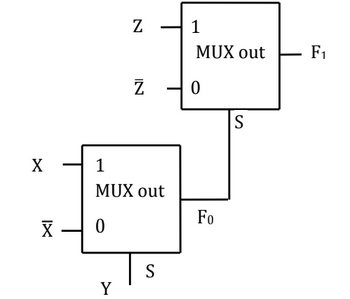
\includegraphics[scale=0.2]{ide.png}
\caption{Multiplexer}
\label{fig:mux}
\end{figure}

\section{ Components}
{
\centering
\begin{tabular}{|c|c|c|}
\hline
Component&Value&Count\\
\hline
Arduino &Uno& 1\\
\hline
LED & Red &1\\
\hline
Resistor&220 Ohm&1\\
\hline
Jumper Wires&-&as-required\\
\hline
\end{tabular}
}
\section{Connections}
\begin{itemize}

\item Connect LED to pin 13 of Arduino with the 220ohm resistor in series
\item Connect 5v and ground points from Arduino to extreme ends of bread board
\item Use D2,D3,D4 pins of Arduino as inputs(x,y,z) referred in Fig.\ref{fig:mux}.  and D13 as output(F)
\end{itemize}
\section{\large Truth table}
{
\centering
\begin{tabular}{|c|c|c|c|c|c|c|}
\hline
$\boldsymbol{x}$&$\boldsymbol{y}$&$\boldsymbol{z}$&$\bar{x}$&$\bar{y}$&$\bar{z}$&$\bar{z+ \bar{x+y}}$\\
\hline
0&0&0&1&1&1&0\\
\hline
0&0&1&1&1&0&1\\
\hline
0&1&0&1&0&1&1\\
\hline
0&1&1&1&0&0&0\\
\hline
1&0&0&0&1&1&1\\
\hline
1&0&1&0&1&0&0\\
\hline
1&1&0&0&0&1&0\\
\hline
1&1&1&0&0&0&1\\
\hline
\end{tabular}
}
$\bar{z+ \bar{(x+y)}}$
\section*{\large Minimization using kmap}
\begin{kvmap}
\kvlist{4}{2}{0,1,0,0,0,1,1,1}{y,z,x}
\bundle[color=red]{1}{0}{1}{1}
\bundle[color=blue]{1}{1}{2}{1}
\bundle[color=green]{2}{1}{3}{1}
\end{kvmap}

\section*{\large Boolean expression}
The boolean expression for \textbf{F} is
\begin{align*}%left aligned equation
%\begin{equation}
%\label{eq:kmap_F}
&F=xy+!(xy)\\
%\end{equation}
%	\section*{\normalsize}
%	The above expression can be further simplified by using boolean postulate that multiplication by  to the second product term in eqn. \eqref{eq:kmap_F}\par
%\begin{equation}
%\label{eq:kmap_F1}
&F=!{x+y}\\
%\end{equation}
%\begin{equation}
%	\label{eq:kmap_F2}
&F1=zs+!(zs)\\
%\end{equation}
%\begin{equation}
%	\label{eq:kmap_F3}
&F1=!{z+s}\\
%\end{equation}
%	the simplified expression for the output F is
%\begin{equation}
%	\label{eq:kmap_F4}
&F1=!{(z+!(x+y)}\\
%\end{equation}
\end{align*}

\section*{\large Software}
Make the connections and connect the arduino the PC via USB.In the location of choice ,type the below commands\\
\subsection{Code Link}
\vspace{5mm}
\begin{table}[h]
    \centering
    \begin{tabular}{|c|}
    \hline 
    https://github.com/vamsi/FWC/tree/main/IDEassigment/code  \\
        \hline
    \end{tabular}
\end{table}
\vspace{5mm}
\begin{enumerate}
\item cd code
\item pio run
\item pio run \-t upload
\end{enumerate}

\end{document}
